\section{Tracing}
\label{sec:Tracing}

COMPSs runtime can generate a post-execution trace of the distributed execution of the application. 
This trace is useful for performance analysis and diagnosis.

A trace file may contain different events as task-execution or file-transfer events among others. 
(In the current release we only support task-execution events and we intend to support file-transfer evens in a future release).

During the execution of the application, an XML file is created at worker nodes to keep track of 
these events. At the end of the execution, all the XML files are merged to get a final trace file.

In the following sections we will explain the command used for tracing, how the events are registered, 
in a process called instrumentation, how to visualize the trace file and make a good analysis of 
performance based on the data shown in the trace.

\subsection{Trace Command}
In order to obtain a post-execution trace file the option ``{\bf --tracing}'' of the 
``{\bf runcompssext}'' command script must be set to ``{\bf true}''. This command is available in 
the system path after COMPSs runtime installation.

Here is the example of the command execution with the tracing option enabled for our Hmmer application.

\begin{lstlisting}[language=bash]
runcompssext --app=hmmerobj.HMMPfam --tracing=true --cline_args="/sharedDisk/Hmmer/smart.HMMs.bin /sharedDisk/Hmmer/256seq   /home/user/out.txt 2 8 -A 222"
\end{lstlisting}
 

\subsection{Application Instrumentation}

The instrumentation is the process that intercepts different events of the application execution 
and keeps log of them. This will cause an overhead in the execution time of the application that 
the user should take into account, but the collected data will be extremely useful for performance 
analysis and diagnosis.

COMPSs runtime uses the Extrae tool from BSC to dynamically instrument the application. 
At worker nodes, in background, Extrae keeps track of the events in an intermediate format 
file (with .mpit extension). In the master, at the end of the execution, Extrae merges the 
intermediate files to get the final trace file, a Paraver format file (.prv). See the visualization 
section in this manual for the Paraver tool.

When instrumenting the application Extrae will output several messages before and after the whole 
user application execution, at the master, and before and after a task execution, at the workers. 
No messages are output during the execution.

\begin{lstlisting}[language=bash]
------------- Executing hmmerobj.HMMPfam ------------------

[   API]  -  Deploying the Integrated Toolkit
[   API]  -  Starting the Integrated Toolkit
[   API]  -  Initializing components

Welcome to Extrae 2.4.3rc4 (revision 311 based on framework/trunk/files/extrae)
Extrae: Generating intermediate files for Paraver traces.
Extrae: Intermediate files will be stored in /home/user/IT/hmmerobj.HMMPfam
Extrae: Tracing buffer can hold 500000 events
Extrae: Tracing mode is set to: Detail.
Extrae: Successfully initiated with 1 tasks

[   API]  -  Ready to process tasks

...
...
...
[   API]  -  No more tasks for app 1
[   API]  -  Stopping IT
[   API]  -  Cleaning

Extrae: Application has ended. Tracing has been terminated.
...

merger: Output trace format is: Paraver
merger: Extrae 2.4.3rc4 (revision 311 based on framework/trunk/files/extrae)
...

[   API]  -  Integrated Toolkit stopped
...

mpi2prv: Selected output trace format is Paraver

mpi2prv: Parsing intermediate files

mpi2prv: Generating tracefile (intermediate buffers of 1342156 events)

mpi2prv: Congratulations! hmmerobj.HMMPfam_compss_trace_1392736225.prv has been generated.

------------------------------------------------------------
\end{lstlisting}

For more information about Extrae please visit the following site: 
\begin{center}
\url{http://www.bsc.es/computer-science/extrae} 
\end{center}


\subsection{Trace Visualization}

Paraver is the BSC tool for trace visualization. Trace events are encoded in Paraver (.prv) 
format by the Extrae tool (see previous section). Paraver is a powerful tool, it can show many 
views of the trace data by mean of different configuration files, and the user can load and 
modify these configuration files or create new ones.

In the following subsections we will see how to load a trace file into Paraver, open the task 
events view by mean of an already predefined configuration file that is provided, and how to 
adjust the view to display the data in the proper way.

For more information about Paraver please visit the following site:

\begin{center}
\url{http://www.bsc.es/computer-sciences/performance-tools/paraver}
\end{center}

\subsubsection{Trace Loading}

The final trace file in Paraver format (.prv) can be found at the application directory under 
the IT directory after the traced-application execution ends. The fastest way to open it is 
calling directly the Paraver command passing to it the trace filename as argument.

\begin{lstlisting}[language=bash]
wxparaver /home/user/IT/hmmerobj.HMMPfam/*.prv
\end{lstlisting}
 
\subsubsection{Configuration File}
In order to open a view with the task events of the application, an already predefined configuration 
file is provided. To open it, just go in the main window to the ``Load Configuration'' option in 
the menu ``File''. The configuration file is under the following path ``/opt/COMPSs/paraver/cfgs/tasks.cfg''. 
After accepting the load of the configuration file, another window will appear to show the view.

\begin{figure}[ht!]
  \centering
    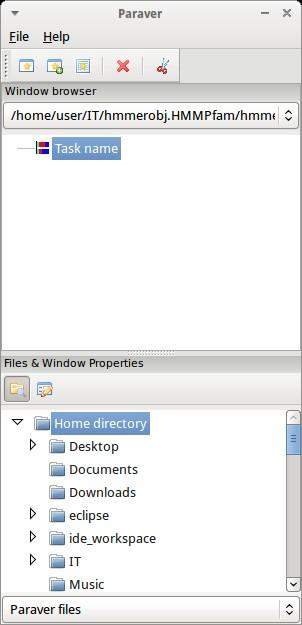
\includegraphics[width=0.45\textwidth]{./Sections/7_Tracing/Figures/1.jpeg}
    %\caption{Caption.}
    %\label{fig:matrix}
\end{figure}

\begin{figure}[ht!]
  \centering
    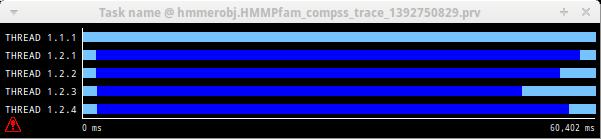
\includegraphics[width=1.0\textwidth]{./Sections/7_Tracing/Figures/2.jpeg}
    %\caption{Caption.}
    %\label{fig:matrix}
\end{figure}

\subsubsection{View Adjustment}
In a Paraver view, a red exclamation sign may appear on the bottom-left corner (see last picture in 
previous section). This means that some little adjustments must be done to view the trace correctly:

\begin{itemize}
 \item Fit window: this will give a better color scale to identify events.
 \begin{itemize}
  \item Right click on the trace window
  \item Chose the option Fit Semantic Scale / Fit Both
 \end{itemize}
\end{itemize}

\begin{figure}[ht!]
  \centering
    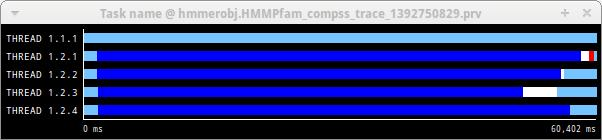
\includegraphics[width=1.0\textwidth]{./Sections/7_Tracing/Figures/3.jpeg}
    %\caption{Caption.}
    %\label{fig:matrix}
\end{figure}

\begin{itemize} 
 \item View Event Flags: This will put a flag whenever an event starts/ends.
\begin{itemize}
 \item Right click on the trace window
 \item Chose the option View / Event Flags
\end{itemize}
\end{itemize}
 
\begin{figure}[ht!]
  \centering
    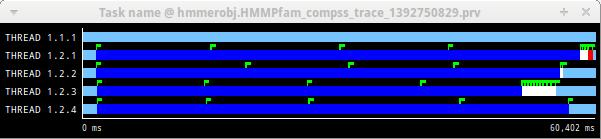
\includegraphics[width=1.0\textwidth]{./Sections/7_Tracing/Figures/4.jpeg}
    %\caption{Caption.}
    %\label{fig:matrix}
\end{figure}

\begin{itemize}
 \item Show Info Panel: This will show an information panel. In the tab ``Colors'' we can see the legend of the colors shown in the view.
 \begin{itemize}
  \item Right click on the trace window
  \item Check the Info Panel option
  \item Select the Colors tab in the panel
 \end{itemize}
\end{itemize}

\begin{figure}[ht!]
  \centering
    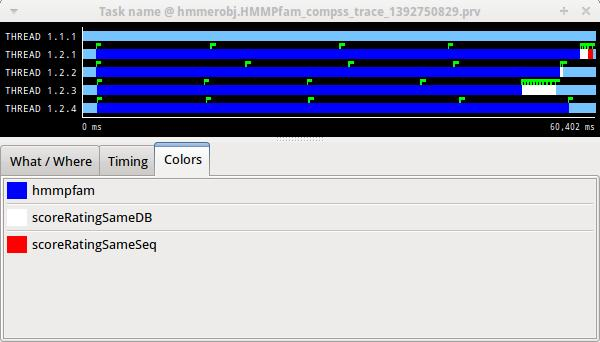
\includegraphics[width=1.0\textwidth]{./Sections/7_Tracing/Figures/5.jpeg}
    %\caption{Caption.}
    %\label{fig:matrix}
\end{figure}

\begin{itemize}
 \item Zoom: In order to understand a trace view better, sometimes it’s a worth thing to zoom into it a little.
 \begin{itemize}
  \item Select a region in the trace window to see that region in detail
  \item And repeat the previous step as many times as needed
  \item The undo-zoom option is in the right click panel
 \end{itemize}
\end{itemize}

\begin{figure}[ht!]
  \centering
    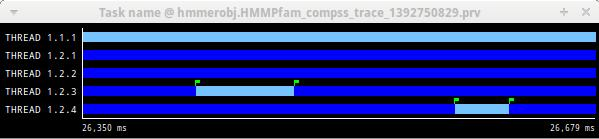
\includegraphics[width=1.0\textwidth]{./Sections/7_Tracing/Figures/6.jpeg}
    %\caption{Caption.}
    %\label{fig:matrix}
\end{figure}

\begin{figure}[ht!]
  \centering
    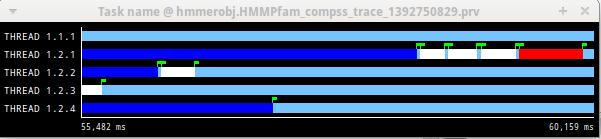
\includegraphics[width=1.0\textwidth]{./Sections/7_Tracing/Figures/6_2.jpeg}
    %\caption{Caption.}
    %\label{fig:matrix}
\end{figure}


\subsection{Trace Interpretation}
In this section we will explain how to interpret a trace view once it has been adjusted as 
described in the previous section.

\begin{itemize}
 \item The trace view has in its horizontal axis the execution time and in the vertical 
       axis one line for the master at the top, and below it, one line for each of the workers.
 \item In a line, the light blue color means idle state, in the sense that there is no event at that time.
 \item Whenever an event starts or ends a flag is shown.
 \item In the middle of an event, the line shows a different color. Colors are assigned depending on the event type.
 \item In the info panel the legend of assigned color to event type is provided.
\end{itemize}

\begin{figure}[ht!]
  \centering
    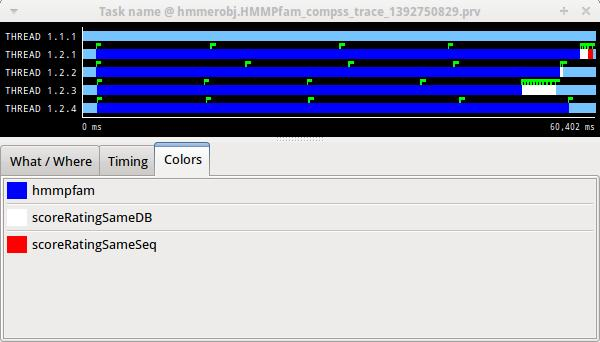
\includegraphics[width=1.0\textwidth]{./Sections/7_Tracing/Figures/7.jpeg}
    %\caption{Caption.}
    %\label{fig:matrix}
\end{figure}

\subsection{Trace Analysis}

In this section, we will give some tips to analyse a COMPSs trace from two points of view 
graphical and numerical.

\subsubsection{Graphical Analysis}

The main concept is that computational events, the task events in this case, must be well 
distributed among all workers to have a good parallelism, and the duration of task events 
should be also balanced, this means, the duration of computational bursts.

\begin{figure}[ht!]
  \centering
    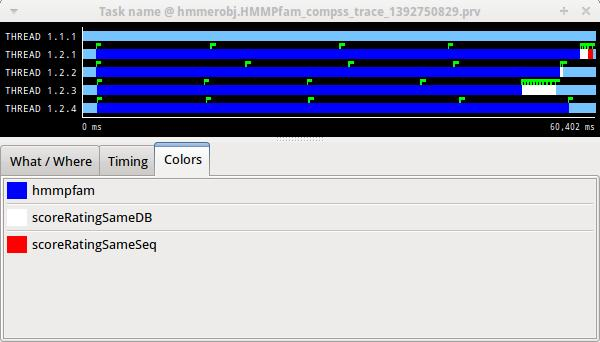
\includegraphics[width=1.0\textwidth]{./Sections/7_Tracing/Figures/8.jpeg}
    %\caption{Caption.}
    %\label{fig:matrix}
\end{figure}

In the previous trace view, all the tasks of type ``hmmpfam'' in dark blue appear to be well 
distributed among the four workers, each worker executes four ``hmmpfam'' tasks.

But some workers finish earlier than the others, worker 1.2.3 finish the first and worker 1.2.1 
the last. So there is an imbalance in the duration of ``hmmpfam'' tasks. The programmer should 
analyse then whether all the tasks process the same amount of input data and do the same thing 
in order to find out the reason of such imbalance.

Another thing to highlight is that tasks of type ``scoreRatingSameDB'' are not equal distributed 
among all the workers. There are workers that execute more tasks of this type than the others. 
To understand better what happens here, let’s take a look to the execution graph and also zoom 
in the last part of the trace.

\begin{figure}[ht!]
  \centering
    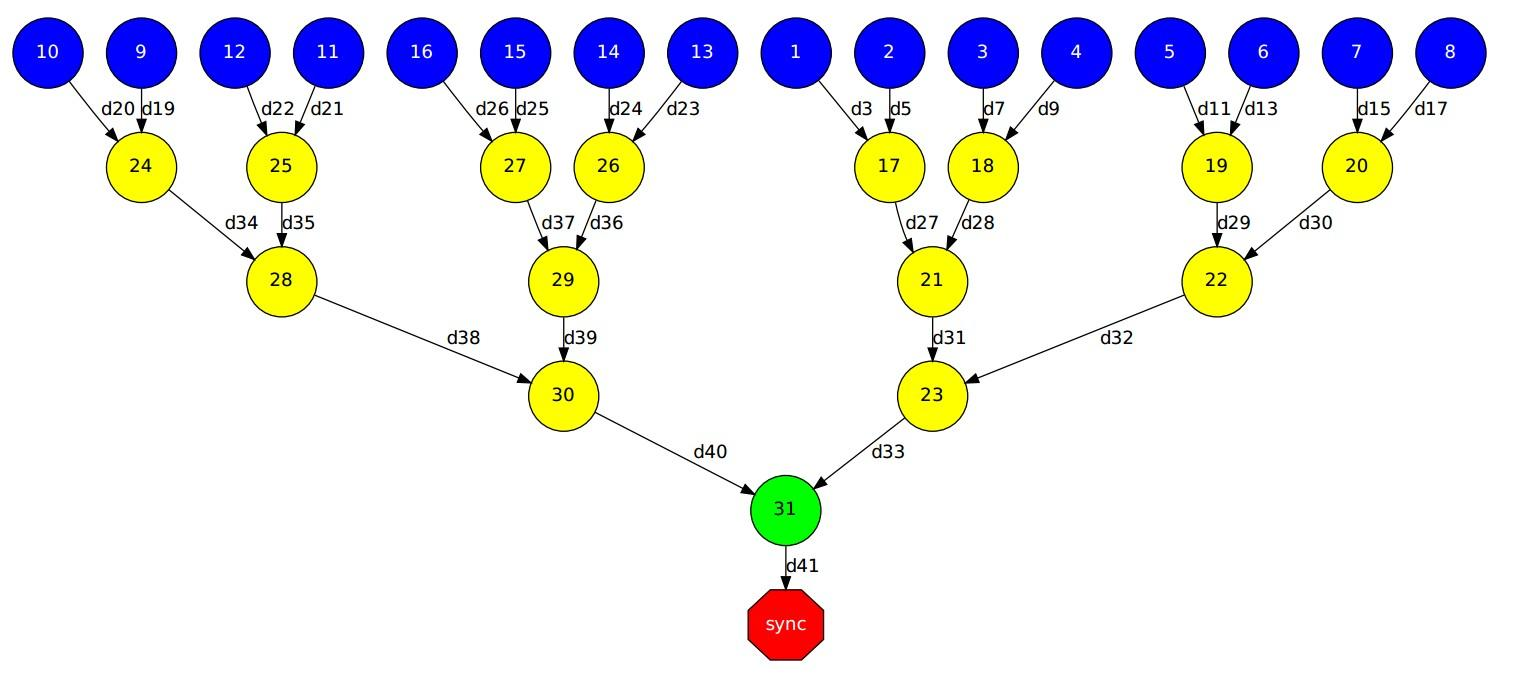
\includegraphics[width=1.0\textwidth]{./Sections/7_Tracing/Figures/9.jpeg}
    %\caption{Caption.}
    %\label{fig:matrix}
\end{figure}

\begin{figure}[ht!]
  \centering
    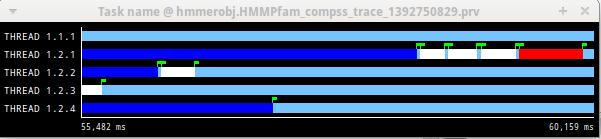
\includegraphics[width=1.0\textwidth]{./Sections/7_Tracing/Figures/10.jpeg}
    %\caption{Caption.}
    %\label{fig:matrix}
\end{figure}


There is only one task of type ``scoreRatingSameSeq''. This task appears in red in the trace 
(and in light-green in the graph). With the help of the graph we see that the ``scoreRatingSameSeq'' 
task has dependences on tasks of type ``scoreRatingSameDB'', in white (or yellow).

When the last task of type ``hmmpfam'' (in dark blue) ends, the last dependences are solved, 
and if we look at the graph, this means going across a path of three dependences of type 
``scoreRatingSameDB'' (in yellow). And because of these are sequential dependences (one depends 
on the previous) no more than a worker can be used at the same time to execute the tasks. 
This is the reason of why the last three task of type ``scoreRatingSameDB'' (in white) are 
executed in worker 1.2.1 sequentially.

\subsubsection{Numerical Analysis}
Here we show another trace from a different parallel execution of the Hmmer program.
 
\begin{figure}[ht!]
  \centering
    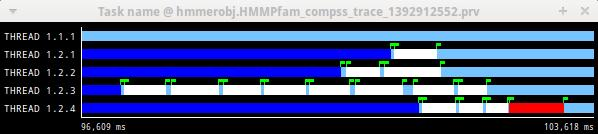
\includegraphics[width=1.0\textwidth]{./Sections/7_Tracing/Figures/11.jpeg}
    %\caption{Caption.}
    %\label{fig:matrix}
\end{figure} 
 
Paraver offers the possibility of having different histograms of the trace events. 
For it just click the ``New Histogram'' button in the main window and accept the 
default options in the ``New Histogram'' window that will appear.

\begin{figure}[ht!]
  \centering
    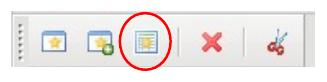
\includegraphics[width=0.5\textwidth]{./Sections/7_Tracing/Figures/12.jpeg}
    %\caption{Caption.}
    %\label{fig:matrix}
\end{figure}

After that, the following table is shown. In this case for each worker, the time spent 
executing each type of task is shown. Task names appear in the same color than in the 
trace view. The color of a cell in a row corresponding to a worker goes in a scale from 
a light-green for lower values to a dark-blue for higher ones. This conforms a color based histogram.

\begin{figure}[ht!]
  \centering
    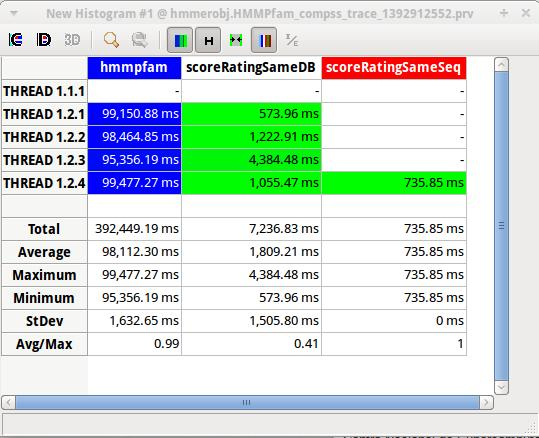
\includegraphics[width=0.8\textwidth]{./Sections/7_Tracing/Figures/13.jpeg}
    %\caption{Caption.}
    %\label{fig:matrix}
\end{figure}
 
The previous table also gives, at the end of each column, some extra statistical 
information for each type of tasks (as the total, average, maximum or minimum values, etc.).

In the window properties of the main window we can change the semantic of the statistics 
to see other factors rather than the time, for example, the number of burst.

\begin{figure}[ht!]
  \centering
    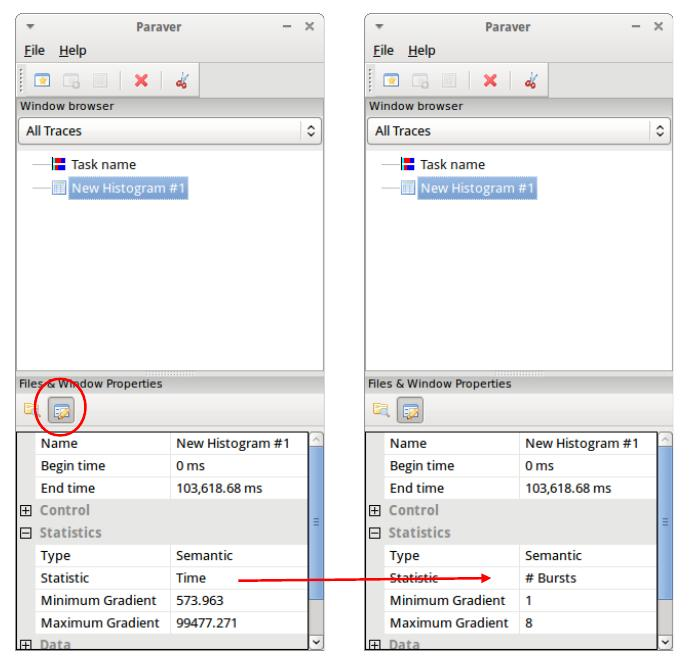
\includegraphics[width=0.8\textwidth]{./Sections/7_Tracing/Figures/14.jpeg}
    %\caption{Caption.}
    %\label{fig:matrix}
\end{figure}

In the same way as before, the following table shows for each worker the number of bursts 
for each type of task, this is, the number or tasks executed of each type. Notice the gradient 
scale from light-green to dark-blue changes with the new values.

\begin{figure}[ht!]
  \centering
    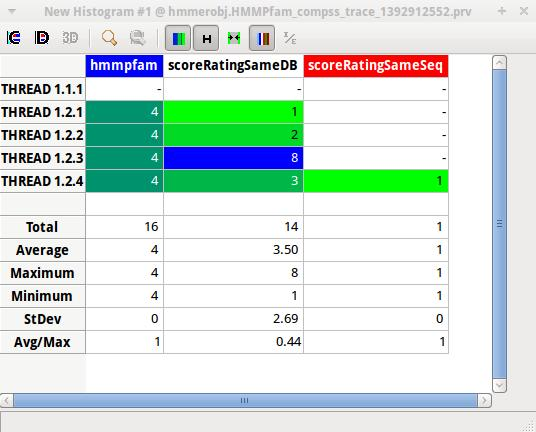
\includegraphics[width=0.8\textwidth]{./Sections/7_Tracing/Figures/15.jpeg}
    %\caption{Caption.}
    %\label{fig:matrix}
\end{figure}

\subsubsection{Other Trace examples}

To end this section, let’s present some other examples of COMPSs traces. COMPSs traces can be 
much complex as the number of workers or tasks grows. Just to illustrate this, the following 
pictures show traces with a greater number of workers and tasks.

\begin{figure}[ht!]
  \centering
    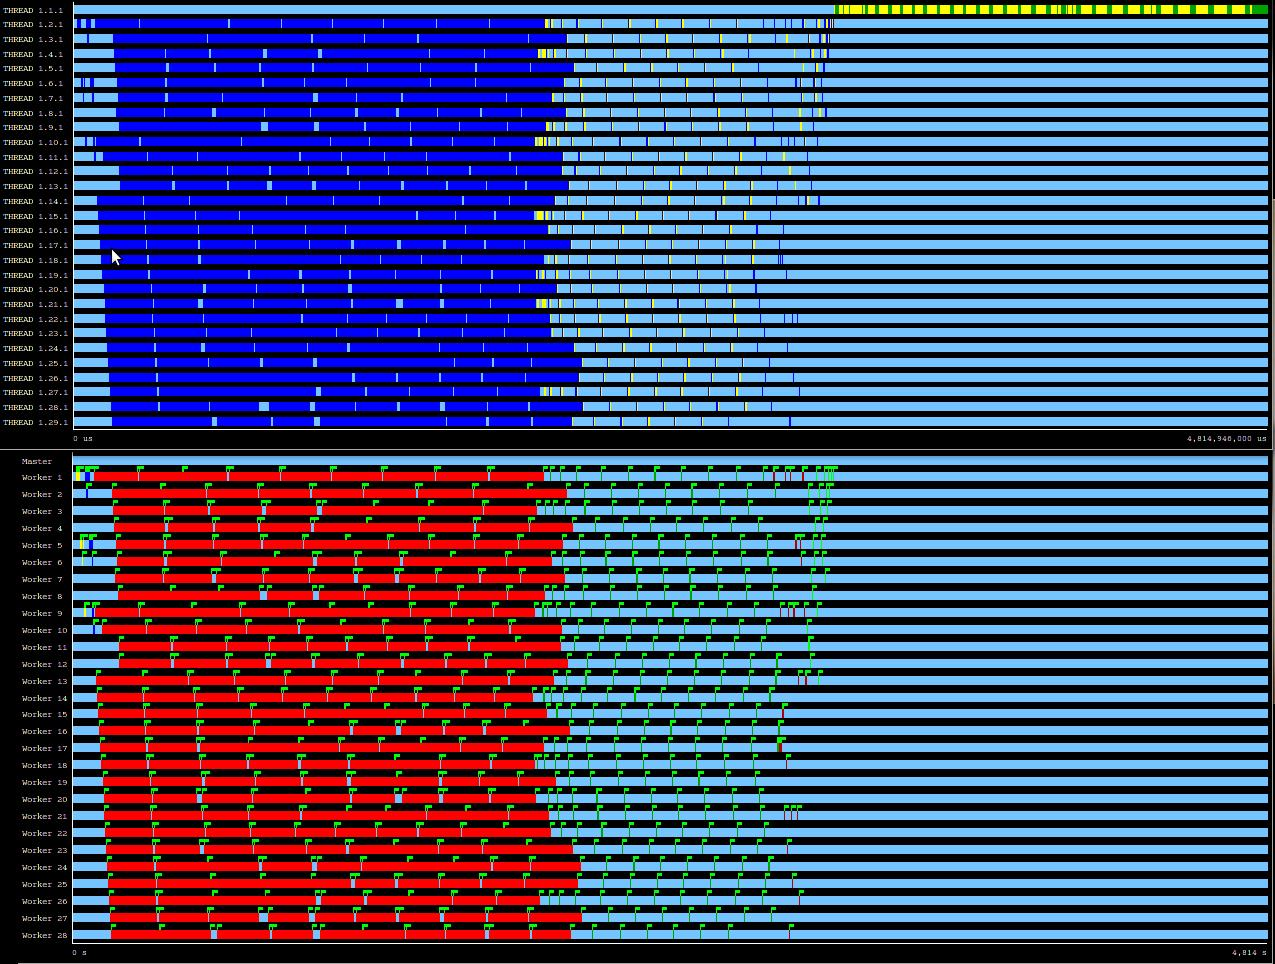
\includegraphics[width=0.91\textwidth]{./Sections/7_Tracing/Figures/16.jpeg}
    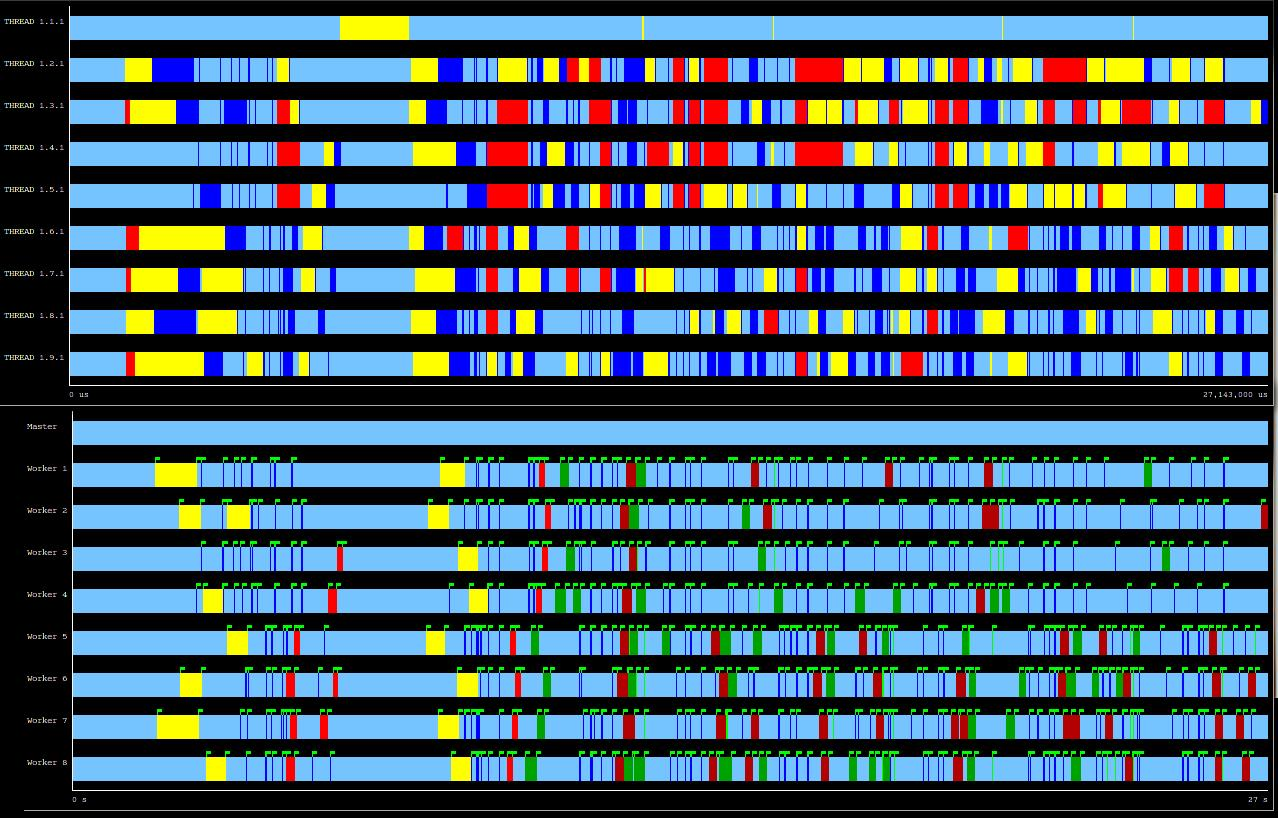
\includegraphics[width=0.91\textwidth]{./Sections/7_Tracing/Figures/16_2.jpeg}
    %\caption{Caption.}
    %\label{fig:matrix}
\end{figure}

